% ----------------------------------------------------------------
% AMS-LaTeX Paper ************************************************
% **** -----------------------------------------------------------
\documentclass{amsart}
\usepackage{graphicx}
% ----------------------------------------------------------------
\vfuzz2pt % Don't report over-full v-boxes if over-edge is small
\hfuzz2pt % Don't report over-full h-boxes if over-edge is small
% THEOREMS -------------------------------------------------------
\newtheorem{thm}{Theorem}[section]
\newtheorem{cor}[thm]{Corollary}
\newtheorem{lem}[thm]{Lemma}
\newtheorem{prop}[thm]{Proposition}
\theoremstyle{definition}
\newtheorem{defn}[thm]{Definition}
\theoremstyle{remark}
\newtheorem{rem}[thm]{Remark}
\numberwithin{equation}{section}
% MATH -----------------------------------------------------------
\newcommand{\norm}[1]{\left\Vert#1\right\Vert}
\newcommand{\abs}[1]{\left\vert#1\right\vert}
\newcommand{\set}[1]{\left\{#1\right\}}
\newcommand{\Real}{\mathbb R}
\newcommand{\eps}{\varepsilon}
\newcommand{\To}{\longrightarrow}
\newcommand{\BX}{\mathbf{B}(X)}
\newcommand{\A}{\mathcal{A}}
% ----------------------------------------------------------------
\begin{document}

\title{Complex Networks  - Spring 2025\\{\bf Homework 5}}%
\author{Instructor: Jia Liu \\ Solution by: Renan Monteiro Barbosa}%
\date{04/30/2025}

%\dedicatory{}%
%\commby{}%
% ----------------------------------------------------------------

\maketitle
% ----------------------------------------------------------------
\begin{itemize}
\item DUE on  04/30/2025 11:59pm C.T.
\item You must finish the homework independently. You may discuss them with your team members and me. 
\item Please name your file as follows: $LastnameInitials-MAP5990quiz1.pdf$.If your name is Alan David Roberts, file name is $RobertsAD-MAP5990quiz1.pdf$.
\item Try to keep the file size less than 4MB.
\item You can resubmit the quiz if you want. Please specify which one is the one to be graded. Otherwise I will grade the most recent version.
\item DO NOT EMAIL me the quiz. All quizzes are submitted via Canvas.
\end{itemize}


\clearpage
\begin{enumerate}

%---------------------------------------------------------------------------------
% ##############################################################################
% Problem 1
% ##############################################################################
\item {\bf These questions will be great preparations for your final project report. You can discuss with your team members but each of you must submit the solutions by yourself.}
\begin{enumerate}
\item Introduce the complex network you will report in your final project:
\begin{enumerate}
\item What is the name of your network?
\item What is the type of the network? Social, biology, information, www, etc?
\item Explain why this network is important.
\item What is the network structure of your network such as node numbers, edge numbers. 
\end{enumerate}

\vspace{1cm}

\textbf{Answers:}

\begin{enumerate}
\item What is the name of your network? \vspace{0.2cm}

Power grid: An undirected, unweighted network representing the topology of the Western States Power Grid of the United States. Data compiled by D. Watts and S. Strogatz and made available on the web here. Please cite D. J. Watts and S. H. Strogatz, Nature 393, 440-442 (1998). \vspace{0.2cm}

\item What is the type of the network? Social, biology, information, www, etc? \vspace{0.2cm}

US Western States Power Grid network to generate and transport electricity \vspace{0.2cm}

\item Explain why this network is important. \vspace{0.2cm}

Electricity is extremely important for the maintenance of the current society we have. \vspace{0.2cm}

\item What is the network structure of your network such as node numbers, edge numbers. \vspace{0.2cm}

Nodes: 4941

Edges: 6594

\end{enumerate}


\vspace{1cm}

\item 
For your references, please include a brief summary of the five references you have cited in the midterm report. Why you want to include these references? What is each reference about? Any past research contribution or related work?
\vspace{1cm}

\textbf{Answers:}



\vspace{1cm}

\item For your final project, what is the methodology you want to use for this project? Explain why you choose this methodology. Keep in mind, here is about the methodology (such as centrality, community detection method, not the experimental steps or network introduction). 
\vspace{0.5cm}

\textbf{Answers:}

We are paying attention to the connected components, network diameter, average path length and the modularity score. \vspace{0.2cm}

We choose these because the represent the best how the electricity is efficently distributed and it is expected the network to follow small world properties as there are realistic limitations about how far its nodes are from each due to geographical limitations and physical limitations on power generation and transport.

\vspace{0.5cm}

\item Summary what you have learned from this project. Any future work? 
\vspace{0.5cm}

\textbf{Answers:}

I learned that a proper research takes a lot more time, for example that are works that have analysed the impact of cascadng failure with proper models representating the physical limitations of the power grid. \vspace{0.2cm}

Also learned that there is no plan or way to prevent a catasthropic disaster given the right conditions arise and that would mean the collapse of the entire power grid living millions in the dark.

\vspace{0.5cm}
\end{enumerate}

\clearpage

% ##############################################################################
% Problem 2
% ##############################################################################

\item Download the power grid network from Neuman's website or Gephi wiki. You may download it from the assignment page. 
\begin{enumerate}
\item Use Gephi to plot the network. Make sure to use centrality and communities so that you can show the properties of the network.
\item choose two different layouts in Gephi to plot the network. 
\item Export the plots and submit the two plots with different layouts. Make sure to use the centrality and communities to show the properties of the network in each plot.
\item Use the resolution 1.0 for the community detection. How many communities you have? 
\item Change the resolution to 0.5 and 5.0, how many communities do you  have for each case?
\end{enumerate}
\vspace{0.5cm}

\textbf{Answers:} \vspace{0.5cm}

% resolution 1.0 for the community detection. 
% How many communities you have? 
% Change the resolution to 0.5 and 5.0
% how many communities do you  have for each case?

With modularity with resolution 1.0 for the community detection. Could detect 36 Communities. \vspace{0.2cm}

Observation: Gephi outputed Modularity of 0.932 with resolution 0.932 \vspace{0.2cm}

With modularity with resolution 0.5 could detect 58 communities. \vspace{0.2cm}

Observation: Gephi outputed modularity of 0.929 with resolution 0.454 \vspace{0.2cm}

With modularity with resolution 5.0 could detect 14 communities. \vspace{0.2cm}
 
Observation: Gephi outputed modularity of 0.901 with resolution 4.836 \vspace{0.2cm}

Layout 1 - Yifan Hu \vspace{0.5cm}

\centering
\begin{minipage}{1\textwidth}
\centering
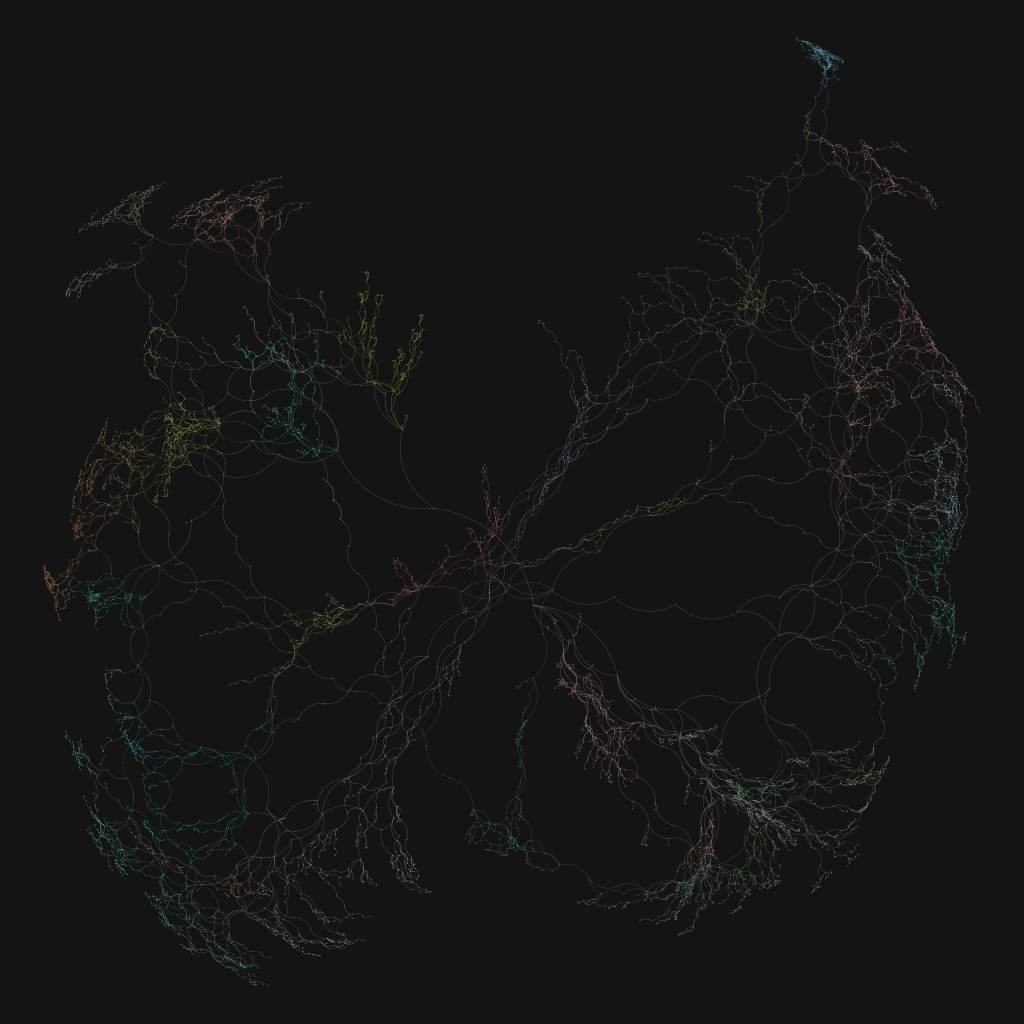
\includegraphics[width=0.8\textwidth]{images/power_layout01_v0.png} % Replace with your image file
\end{minipage}

\vspace{0.5cm}

Layout 2 - Forced Atlas 2 \vspace{0.5cm}

\centering
\begin{minipage}{1\textwidth}
\centering
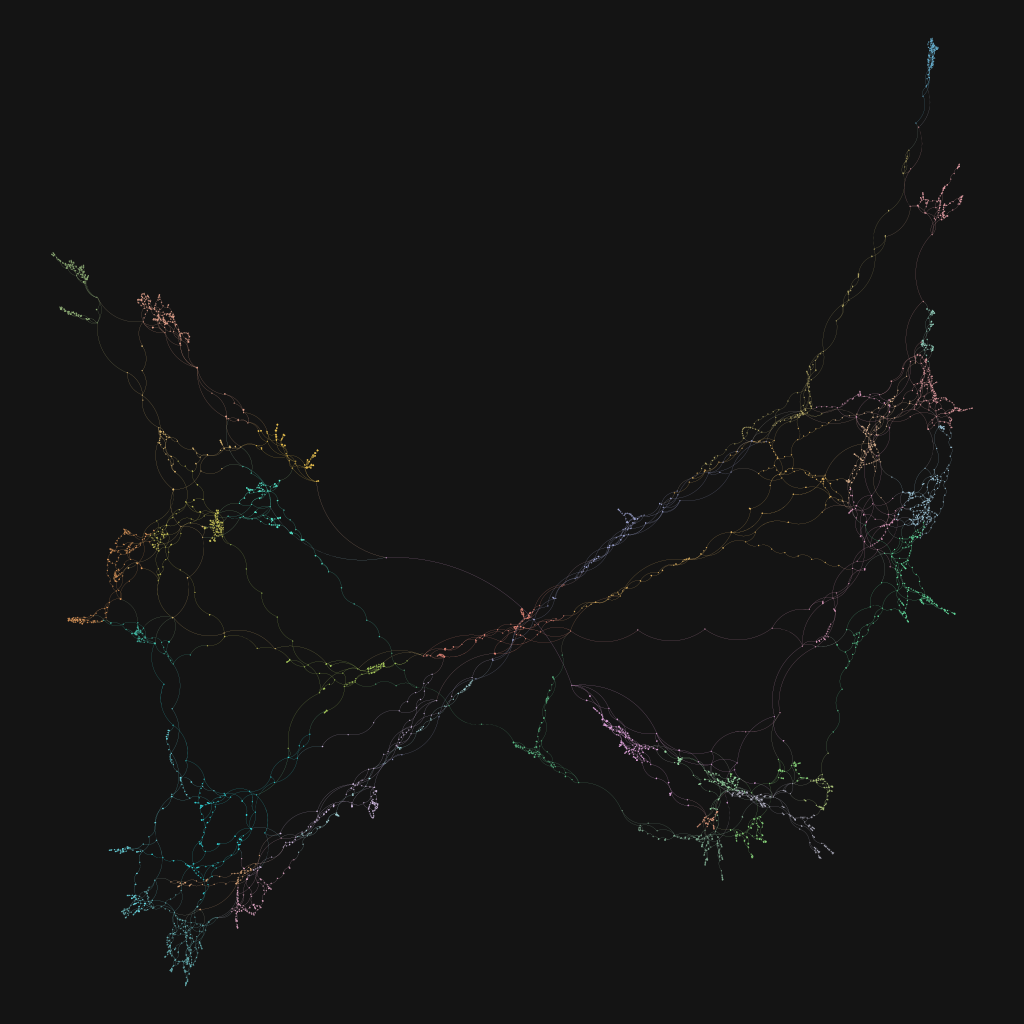
\includegraphics[width=0.8\textwidth]{images/power_layout02_v0.png} % Replace with your image file
\end{minipage}

\vspace{1cm}

% ##############################################################################
% Problem 3
% ##############################################################################

\item  Repeat the same steps in the previous problem on the network from your final project. Make sure to use centrality and communities so that you can show the properties of the network.
% ----------------------------------------------------------------

\end{enumerate}

\textbf{Answers:} \vspace{0.5cm}

% resolution 1.0 for the community detection. 
% How many communities you have? 
% Change the resolution to 0.5 and 5.0
% how many communities do you  have for each case?

With modularity with resolution 1.0 for the community detection. Could detect 36 Communities. \vspace{0.2cm}

Observation: Gephi outputed Modularity of 0.932 with resolution 0.932 \vspace{0.2cm}

With modularity with resolution 0.5 could detect 58 communities. \vspace{0.2cm}

Observation: Gephi outputed modularity of 0.929 with resolution 0.454 \vspace{0.2cm}

With modularity with resolution 5.0 could detect 14 communities. \vspace{0.2cm}
 
Observation: Gephi outputed modularity of 0.901 with resolution 4.836 \vspace{0.2cm}


Layout 1 - Yifan Hu \vspace{0.5cm}

\centering
\begin{minipage}{1\textwidth}
\centering
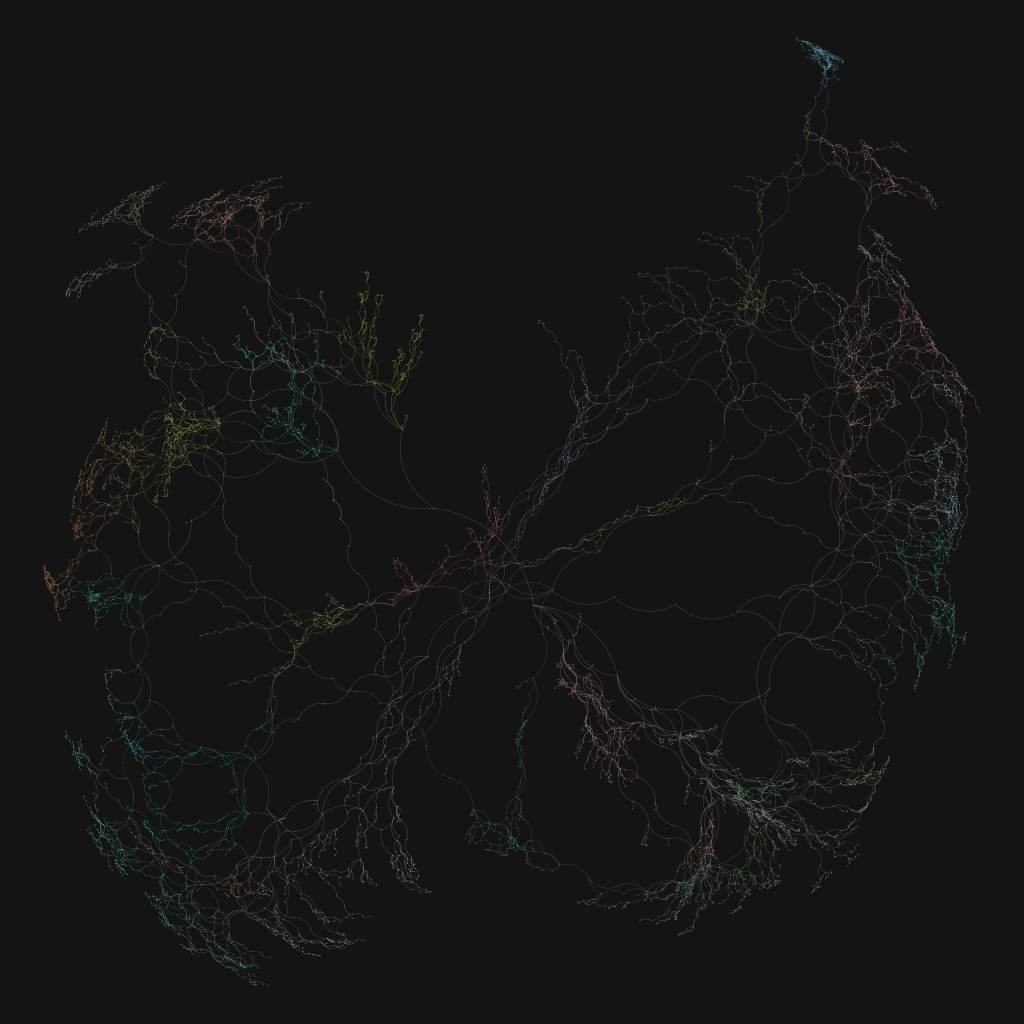
\includegraphics[width=0.8\textwidth]{images/power_layout01_v0.png} % Replace with your image file
\end{minipage}

\vspace{0.5cm}

Layout 2 - Forced Atlas 2 \vspace{0.5cm}

\centering
\begin{minipage}{1\textwidth}
\centering
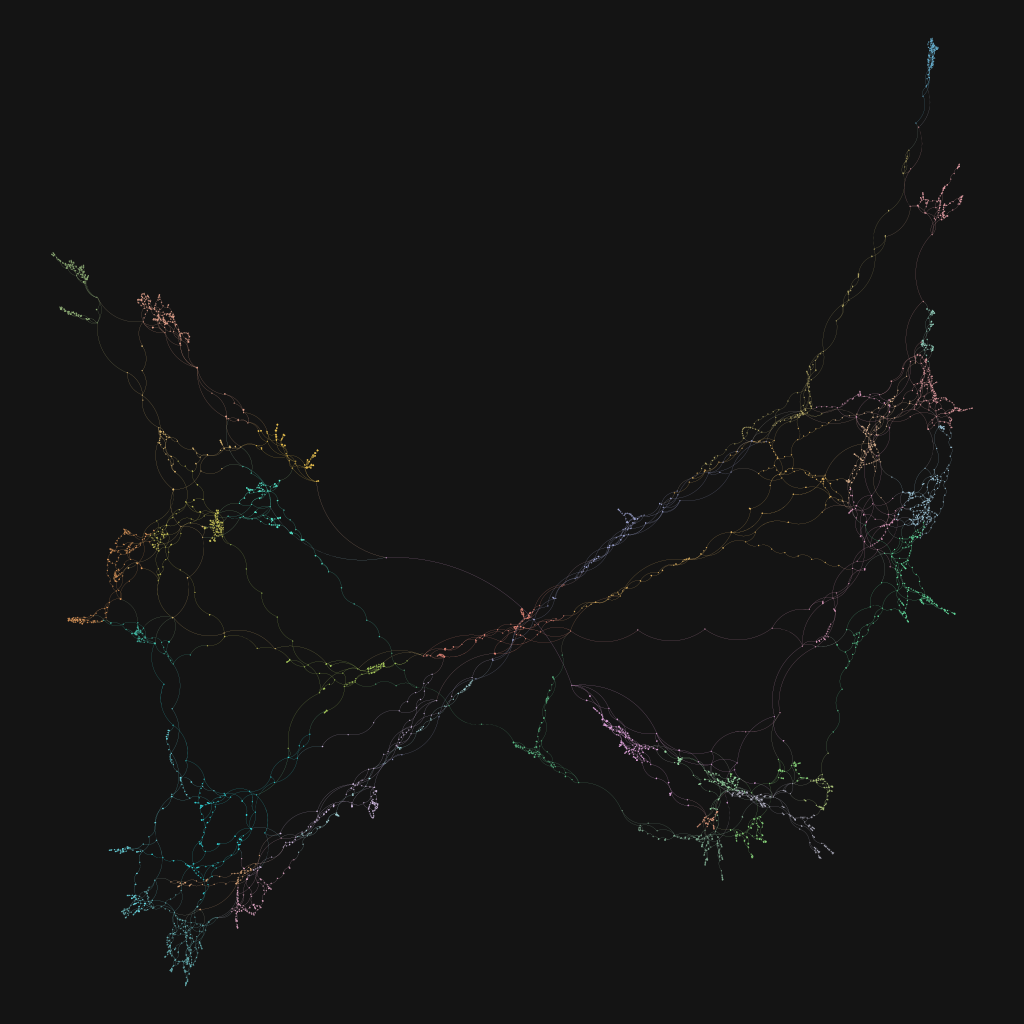
\includegraphics[width=0.8\textwidth]{images/power_layout02_v0.png} % Replace with your image file
\end{minipage}

\end{document}
% ----------------------------------------------------------------
